% 2007 年浙江卷理科第 19 题：EA、DB 均垂直于平面 ABC，AC⊥BC，M 为 AB 中点。
%   按 AC=BC=2、AE=1、BD=2 的示意比例绘制。
% 来源 PDF：gaokaomath-src/普通高考/2007/2007浙江理.pdf
% SHA-256：31c1d0d79ba11a3644a27b5ee3781f52caaf831209e8da63ddd8d7019cd06995
% 原页：2007浙江理.pdf 第 2 页（A3 三栏）第 1 栏，书页码 418。
% 重绘依据：按原页 C、A、B 底面与 E、D 的竖直位置重绘。
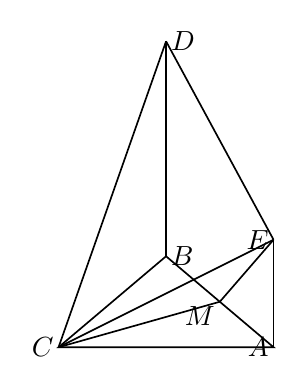
\begin{tikzpicture}[scale=1.05, semithick,
  every node/.style={inner sep=1.5pt}]

  \coordinate (C) at (0,0);
  \coordinate (A) at (2.6,0);
  \coordinate (B) at (1.3,1.1);
  \coordinate (E) at (2.6,1.3);
  \coordinate (D) at (1.3,3.7);
  \coordinate (M) at (1.95,0.55);

  % 底面
  \draw (C) -- (A) -- (B) -- cycle;
  % 竖直线
  \draw (A) -- (E);
  \draw (B) -- (D);
  % 上方连线
  \draw (E) -- (D);
  \draw (E) -- (C);
  \draw (D) -- (C);
  % 中点 M 相关
  \draw (C) -- (M);
  \draw (E) -- (M);

  \node[left] at (C) {$C$};
  \node[left] at (A) {$A$};
  \node[right] at (B) {$B$};
  \node[left] at (E) {$E$};
  \node[right] at (D) {$D$};
  \node[below left] at (M) {$M$};
\end{tikzpicture}
